
\def\problemset#1#2{
\begin{center}
\framebox{\framebox{\vspace{0.5in}
  \parbox{12cm}{\bf
    Gaurav Nanda \hfill Homework \#3\\
    Natural Language Processing \hfill #2, 2014}
  }}\vspace{0.05in}
\end{center}
}

\documentclass[11pt]{article}
\usepackage{fullpage}
\usepackage{algorithm}
\usepackage{algpseudocode}
\usepackage{hyperref}
\usepackage{footnote}
\usepackage{graphicx}

\setlength{\parindent}{0in}
\setlength{\parskip}{2mm}

%\setlength{\oddsidemargin}{-0.5cm}
%\setlength{\evensidemargin}{-0.5cm}
%\setlength{\textwidth}{18cm}

%\setlength{\topmargin}{-1.7cm}
%\setlength{\textheight}{25cm}
\begin{document}
\problemset{1}{March 29}

\section{Implementation}

\subsection {Domain Adaptation Parser}

This parser provides basic functionality to train with the seed data, annotate a pool of self-training data and combine the seed and self-trained data to create a new model. Further, performance of the new model is measured using the test dataset.

Seed data, self-training data and test dataset are passed as arguments to the parser. If there is no self-training data, pass "NOADAPTION" as an argument. Another optional argument has been provided to enable the multi-threading. Parsing of the self-training data is done in parallel using the number of threads argument.

Memory Tree Bank is used to combine self-training and seed data into the new model. Also, I am using \textit{parseMultiple} function in \textit{LexicalizedParser} class, which internally call \textit{parse} method to convert  input sentence to a Tree. However, there was an exceptional case that I handled for the sentences which are not parsed properly. If there is an exception while parsing, Parser add "X" as its root. Therefore, before adding self-trained trees back to the new model, we filter out all trees with "X" at its root. 

\subsection {Pre-Processors}

There are two preprocessors implmented to produce various input files required for the Domain Adaption Parser. 

First, Sentence Extractor, takes input location, output location and maximum number of sentences to be generated. Therefore, for WSJ we provide 35000 as max number and it generates various splits in range of 1 and 35,000 separted by 1000. Therefore, we go over input file only once.

Second, Split Brown, reads in each genre and takes 90-10 split for each of them. Further, all 90s are clubbed together to form training file and rest are put in test file. 

\section {Experiments}

Severals experiments were run in order to see the performance of domain adaptation or transfer learning.
Here is the discussion of the experiments we ran:

\subsection {Varying size of WSJ seed}

Here we performed three different tests while varying the nunber of sentences in WSJ seed. Tests include unsupervised domain adaptation by normal training on WSJ, self-training on Brown, and then testing on Brown, normal training on WSJ and testing on Brown and normal training and testing on WSJ. Training dataset is 90\% of brown corpus and rest of 10\% is test corpus.

\begin{figure}[ht!]
\centering
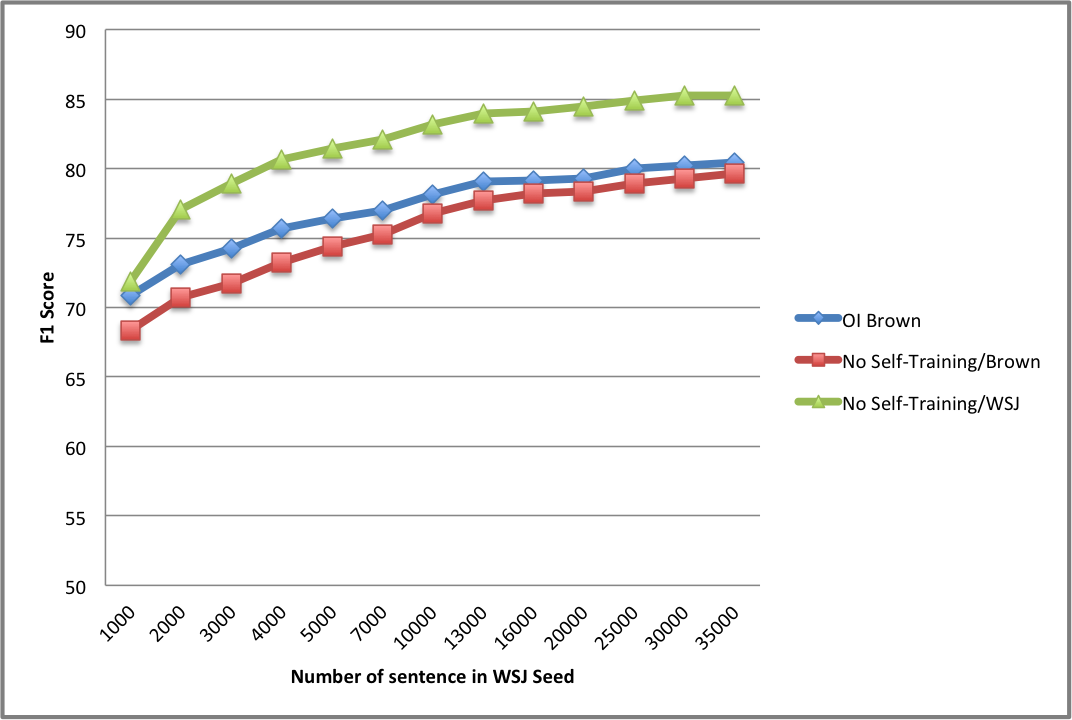
\includegraphics[width=140mm]{exp1.png}
\caption{Learning curve of F1 score as a function of number of sentences in the seed set. (Blue:- Unsupervised domain adaptation by normal training on WSJ, self-training on Brown, and then testing on Brown). (Red:- Normal training on WSJ and testing on Brown). (Green:- Normal training and testing on WSJ).}
\label{accuracy}
\end{figure}

\textbf {In-domain testing Vs. out-of-domain testing}

Without any domain adaptation, on average, there is 7.57\% drop in F1 score from in-domain testing to out-domain testing.

\textbf {Impact of unsupervised domain adaptation on out-of-domain testing}

On average there is an increase of 2.16\% when we do unsupervised domain adaptation. However, percentage increase decreases, as we keep on increasing the seed-data. For instance, for 1000 seed sentences, percentage increase is 3.67\% and for 35000 percentage increase is only 0.96\%. This signifies the impact of domain adaptation is less when we have large amount of seed data.

\textbf {Impact of seed size.}

As we keep on increasing the seed size, F1 score keeps on increasing. However, as expected, percentage increase keeps on going lower with larger seed size. For example, for domain adaptation OI case, percentage increase from 1000 to 2000 sentence is 3.10\%. However, percentage increase from 30,000 to 35,000 is only 0.27\%. 

Here is the table having all the values for this experiment:

\begin{figure}[ht!]
\centering
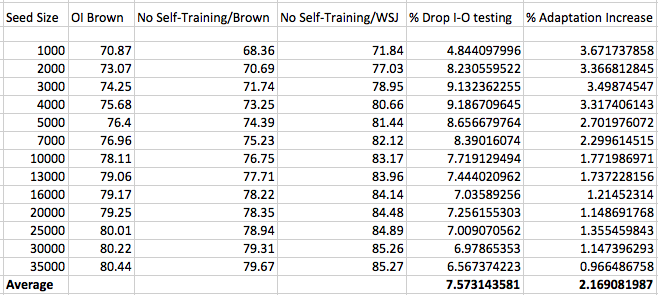
\includegraphics[width=140mm]{exp1-snapshot.png}
\caption{Table showing F1 scores as a function of number of sentences in the seed set. }
\label{accuracy}
\end{figure}

Column-1 shows the seed size. Column-2 shows F1 score, where, normal training on WSJ, self-training on Brown, and then testing on Brown. Column-3 shows F1 score, with normal training on WSJ and testing on Brown. Column-4 shows F1 score, where, normal training and testing on WSJ. Column-5 represents percentage drop in F1 score from in-domain to out-domain testing. Column-6 shows percentage increase in F1 score with unsupervised domain adaptation on baseline out-of-domain testing.

\newpage

\subsection {Varying size of self-supervised Brown training sets.}

Here, we fixed the WSJ seed size to 10,000 sentences and varied the size of self-supervised training data. Increasing size of self-supervised training data hardly increases F1 score. For 1000 sentences, F1 score is 76.91 and for 21,000 sentences, F1 score is 78.01. There is very little increase with increase in count of training data size.

\begin{figure}[ht!]
\centering
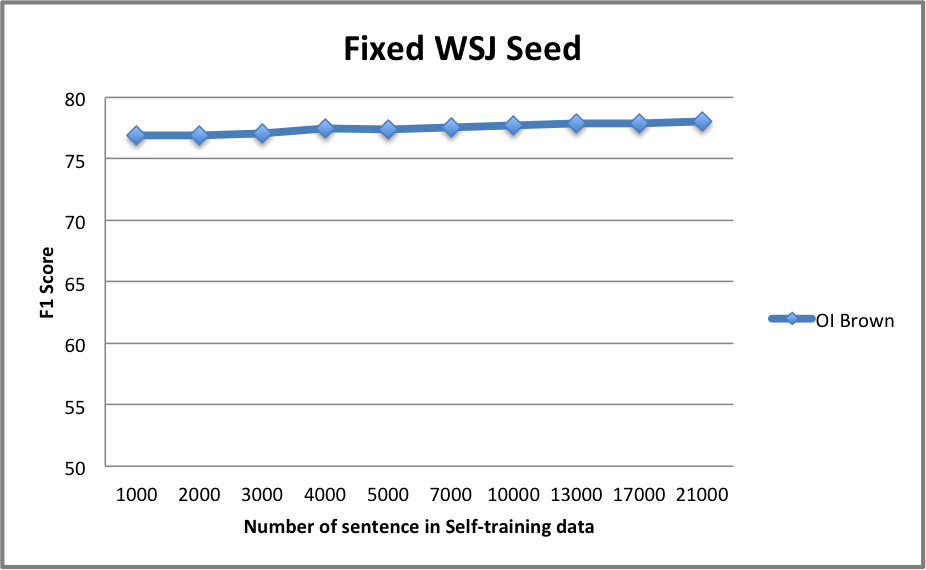
\includegraphics[width=140mm]{exp2.png}
\caption{Table showing F1 scores as a function of number of sentences in the seed set. }
\label{accuracy}
\end{figure}

\newpage
\subsection {Varying size of Brown seed.}

Here we perform the same three tests, as we had performed while varying the WSJ seed size. However, we use previous 90\% Brown data as the seed set, WSJ sections 02-22 as the self-training data and WSJ section 23 as the test set.

\begin{figure}[ht!]
\centering
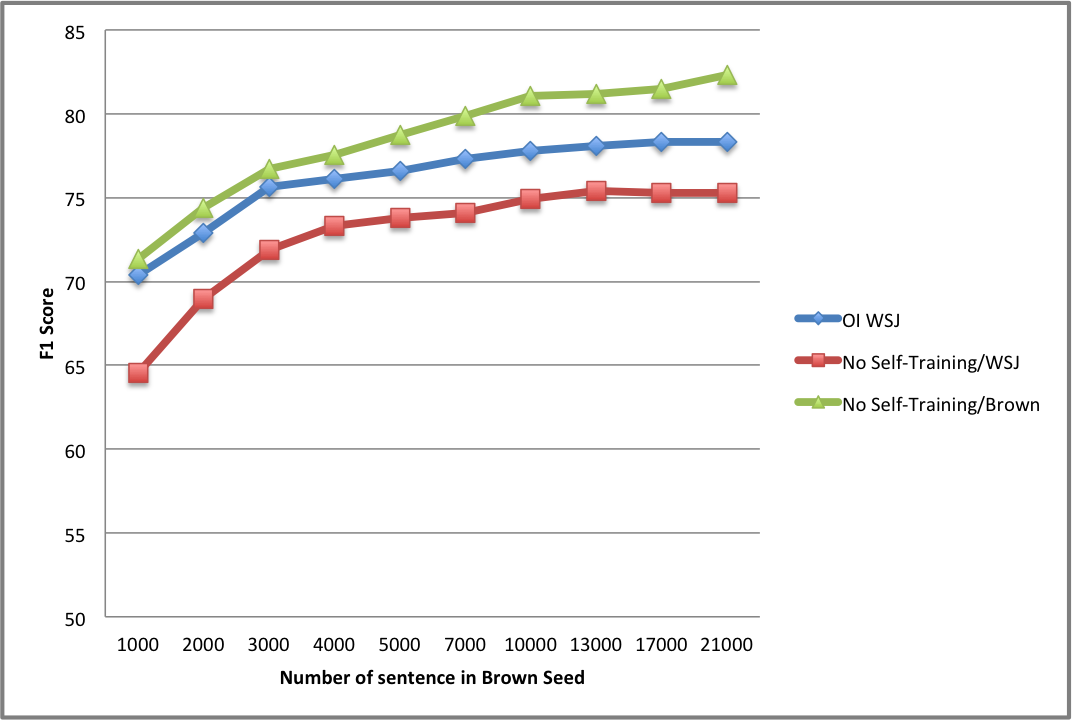
\includegraphics[width=140mm]{exp3.png}
\caption{Learning curve of F1 score as a function of number of sentences in the seed set. (Blue:- Unsupervised domain adaptation by normal training on Brown, self-training on WSJ, and then testing on WSJ). (Red:- Normal training on Brown and testing on WSJ). (Green:- Normal training and testing on Brown).}
\label{accuracy}
\end{figure}

\textbf {Impact of inverting the "source" and "target"}

Most of the observations are similar to our previous test for WSJ. However, if we observe the graph carefully, gap between blue and red lines have increased. This tells us that percentage increase of F1 values with self-trained data is higher in comparison to previous WSJ test. 

This means that, domain adaptation is more helpful for WSJ data set in comparison to Brown data set. I surmise this happens because WSJ is not a diverse dataset and has data only pertaining to the financial world. Therefore, as the term "domain adaptation" suggests, when addition of self-trained WSJ data, F1 score on test data increases. Moreover, this increase is higher in comparison to self-adaptation on Brown data as that is a diverse data set.

\textbf {In-domain testing Vs. out-of-domain testing}

Without any domain adaptation, on average, there is 7.3\% drop in F1 score from in-domain testing to out-domain testing. This number is roughly similar to number before inversion.

\textbf {Impact of unsupervised domain adaptation on out-of-domain testing}

On average there is an increase of 4.73\% when we do unsupervised domain adaptation. However, percentage increase decreases, as we keep on increasing the seed-data. For instance, for 1000 seed sentences, percentage increase is 9.08\% and for 21000 percentage increase is 3.98\%. This signifies the impact of domain adaptation is less when we have large amount of seed data. 

These numbers as we discussed earlier highlight the benefit of doing domain adaptation for WSJ in comparison to a diverse dataset like Brown.

\textbf {Impact of seed size.}

As we keep on increasing the seed size, F1 score keeps on increasing. However, as expected, percentage increase keeps on going lower with larger seed size. For example, for domain adaptation OI case, percentage increase from 1000 to 2000 sentence is 3.56\%. However, percentage increase from 17,000 to 21,000 is almost 0. 

Here is the table having all the values for this experiment:

\begin{figure}[ht!]
\centering
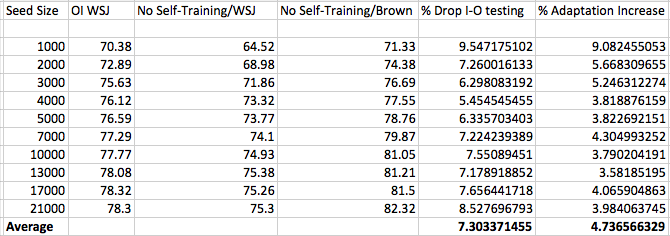
\includegraphics[width=140mm]{exp3-snapshot.png}
\caption{Table showing F1 scores as a function of number of sentences in the seed set. }
\label{accuracy}
\end{figure}

Column-1 shows the seed size. Column-2 shows F1 score, where, normal training on Brown, self-training on WSJ, and then testing on WSJ. Column-3 shows F1 score, with normal training on Brown and testing on WSJ. Column-4 shows F1 score, where, normal training and testing on Brown. Column-5 represents percentage drop in F1 score from in-domain to out-domain testing. Column-6 shows percentage increase in F1 score with unsupervised domain adaptation on baseline out-of-domain testing.

\newpage

\subsection {Varying size of self-supervised WSJ training sets.}

Here, we fixed the Brown seed size to 10,000 sentences and varied the size of self-supervised WSJ training data. Increasing size of self-supervised training data hardly increases F1 score. For 1000 sentences, F1 score is 75.82 and for 35,000 sentences, F1 score is 77.86. There is very little increase with increase in count of training data size.

\begin{figure}[ht!]
\centering
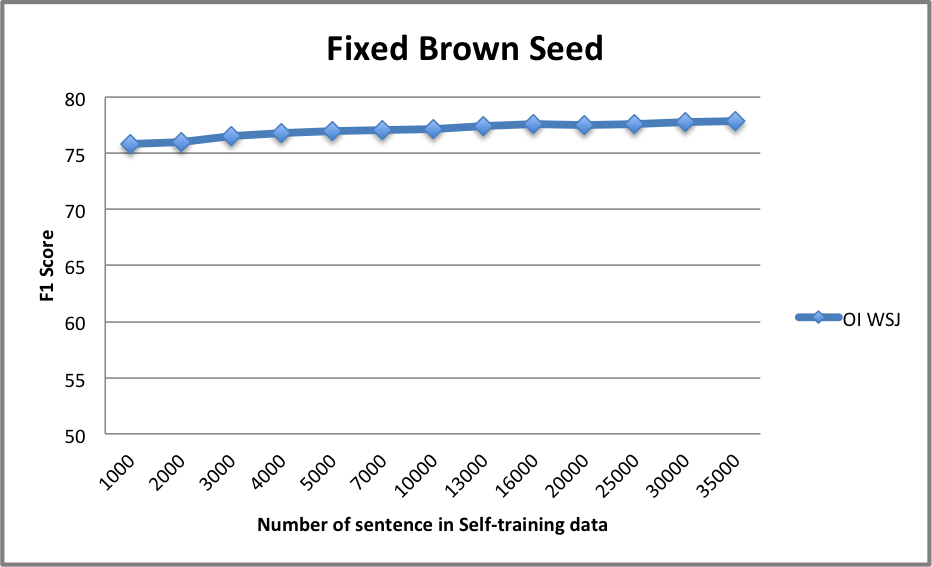
\includegraphics[width=140mm]{exp4.png}
\caption{Table showing F1 scores as a function of number of sentences in the seed set. }
\label{accuracy}
\end{figure}

\section{Comparison with Reichart and Rappoport paper for OI setting}

Our results corroborate with the results of paper. As discussed in the paper, there is consistent increase in the F1 score with self-training data for the OI setting. As we also observed, percentage increase in F1 number is higher for smaller seed data. This implies that, if we have less manually annotated data, we can self-train using un-annotated data from test domain, which would help increase the F1 score.

\end{document}

